\documentclass[11pt]{article}
\usepackage[margin=0.88in]{geometry}
\usepackage[T1]{fontenc}
\usepackage{lmodern,microtype,amsmath,amssymb,booktabs,array,xcolor,fancyhdr}
\usepackage{tikz}
\usetikzlibrary{arrows.meta,positioning,calc,fit,backgrounds}
\usepackage[font=small,labelfont=bf]{caption}
\usepackage[colorlinks=true,urlcolor=blue!45!black,linkcolor=blue!45!black]{hyperref}
\definecolor{ink}{RGB}{24,47,65}
\definecolor{teal}{RGB}{20,106,112}
\definecolor{amber}{RGB}{166,105,27}
\pagestyle{fancy}\fancyhf{}\fancyhead[L]{\small\sffamily SALTy-rn / Unbounded equivalence}
\fancyhead[R]{\small\sffamily Technical report}\fancyfoot[C]{\thepage}
\setlength{\headheight}{14pt}
\setlength{\parindent}{1.1em}\setlength{\parskip}{3pt}
\setlength{\textfloatsep}{14pt plus 3pt minus 3pt}
\newcommand{\code}[1]{{\small\texttt{#1}}}
\newcommand{\neon}{\mathsf{NEON}}
\newcommand{\rvv}{\mathsf{RVV}}
\tikzset{box/.style={draw=ink!65,rounded corners=2pt,align=center,fill=ink!3,inner sep=7pt,font=\small},arr/.style={-{Stealth[length=2mm]},thick,draw=ink!75}}
\begin{document}
\thispagestyle{empty}
\begin{center}
{\sffamily\color{ink}\LARGE Unbounded equivalence for SALTy-rn\par}
\vspace{5pt}
{\large A shared semantic model for NEON and RVV kernels\par}
\vspace{7pt}
{\small Technical report\quad $\cdot$\quad 14 October 2026}
\end{center}
\begin{abstract}
A SIMD translation can agree with its source on many tested sizes and still fail at a tail, an unusual shift count, or a different vector length. This report describes a Lean 4 framework for proving that complete NEON and RISC-V Vector (RVV) intrinsic kernels have the same observable behavior for every admitted call. Both programs execute in a shared byte-addressed model; independent termination and functional-correctness proofs connect them to one reference result. Loop induction removes the fixed execution bound used by the existing symbolic checks. The development establishes whole-function results for 11 of 36 implemented pairs and records 17 translation repairs, with separate evidence for each. The remaining 25 pairs are unproved; four absent or empty targets are excluded. The guarantees depend on explicit caller contracts and a trusted source-extraction bridge. They concern intrinsic C programs, not compiled binaries.
\end{abstract}

\section{Why matching lanes is not enough}
SALTy-rn translates kernels written with ARM NEON intrinsics into kernels using RVV intrinsics. NEON code commonly processes a fixed number of elements per iteration. RVV code instead selects an \emph{active vector length}, denoted $\mathit{vl}$, according to the remaining work and the available vector capacity. \emph{VLEN} is the hardware vector-register width in bits; it is not the number of active elements. The chosen element width and register grouping determine how many elements fit.

At the level of one element, a translation may look straightforward. A signed-byte clamp, for example, computes
\[
 f(x)=\min(\max(x,\ell),u),\qquad \ell\le u,
\]
where $x$, $\ell$, and $u$ are signed 8-bit values. Proving that both instruction sequences implement $f$ is necessary, but it does not prove that the complete functions agree. The loops must cover exactly the requested elements, stores must go to the right addresses, and every load must be valid. Different iteration schedules can also change whether a store overwrites input that has yet to be read.

Figure~\ref{fig:clamp} shows the issue for a call with 13 elements. The source handles eight elements, then reads another eight for a five-element tail. The target can process all 13 active elements in one iteration. Both must write the same 13 answers and leave every other byte unchanged, even though their reads and instruction counts differ.

\begin{figure}[htbp]
\centering
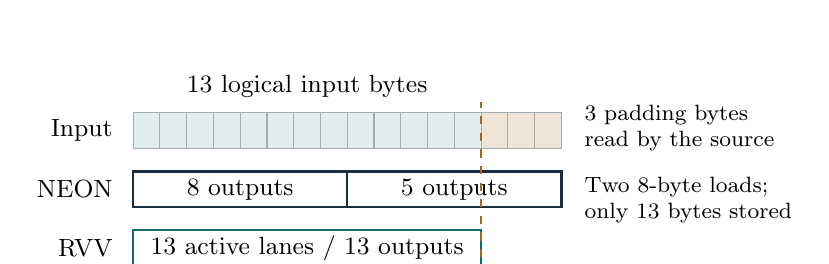
\begin{tikzpicture}[x=0.34cm,y=0.65cm,font=\small]
\node[anchor=east] at (-0.4,2) {Input};
\node[anchor=east] at (-0.4,0.85) {NEON};
\node[anchor=east] at (-0.4,-0.3) {RVV};
\foreach \i in {0,...,15} {
 \ifnum\i<13 \fill[teal!12] (\i,1.65) rectangle +(1,0.7);
 \else \fill[amber!18] (\i,1.65) rectangle +(1,0.7);\fi
 \draw[ink!40] (\i,1.65) rectangle +(1,0.7);
}
\draw[ink,thick] (0,0.5) rectangle (8,1.2);
\draw[ink,thick] (8,0.5) rectangle (16,1.2);
\node at (4,0.85) {8 outputs};
\node at (12,0.85) {5 outputs};
\draw[teal,thick] (0,-0.65) rectangle (13,0.05);
\node at (6.5,-0.3) {13 active lanes / 13 outputs};
\draw[dashed,amber,thick] (13,-0.8)--(13,2.55);
\node[anchor=south] at (6.5,2.45) {13 logical input bytes};
\node[anchor=west,align=left,font=\footnotesize] at (16.5,2.05) {3 padding bytes\\read by the source};
\node[anchor=west,align=left,font=\footnotesize] at (16.5,0.65) {Two 8-byte loads;\\only 13 bytes stored};
\end{tikzpicture}
\caption{An actual clamp execution shape at length 13. The RVV register group has capacity for all 13 elements. The source tail reads three padding bytes in this example; the general caller contract reserves seven. Padding is readable but is not part of the output.}
\label{fig:clamp}
\end{figure}

The framework addresses this whole-function problem through three layers: a common meaning of observable behavior, a reusable machine and instruction model, and per-family caller contracts and reference results. Kernel-specific mathematics remains in the specifications; it does not become a new instruction semantics for each kernel. The central result is a reusable proof architecture and a precisely delimited collection of established theorems, rather than a claim that all translations are already verified.

\section{The guarantee and its assumptions}
\subsection{What two executions must agree on}
For the proved kernels, the returned observation is the entire final memory. These C functions return void, so there is no additional scalar result. Memory maps 64-bit addresses to bytes and also records read and write permissions. Equality of final observations therefore says more than equality of output arrays: bytes outside the output footprint and both permission maps are preserved as specified.

The observation deliberately omits intermediate registers, instruction counts, memory-read traces, timing, floating-point exception flags, and saturation flags. This matters even for clamp: the source can compute on padded lanes that the target never activates. Requiring all intermediate effects to agree would rule out otherwise valid changes in vectorization.

A machine has a deterministic next-step function. Each step either continues with a new state or produces a terminal outcome: a returned observation or a fault. An executable function, $\mathit{run}(n,s)$, follows at most $n$ steps from state $s$. Exhausting this \emph{fuel} returns no outcome; it does not mean that the program diverges. We write
\[
 M,s\Downarrow o\quad\Longleftrightarrow\quad
 \exists n.\ \mathit{run}_M(n,s)=\mathsf{some}(o).
\]
A state diverges when no finite fuel produces a terminal outcome. Because the transition function is total and deterministic, terminal outcomes are unique and persist when more fuel is supplied.

Let $i$ contain the call arguments, initial memory, and vector configuration. Let $P(i)$ be the caller contract and $\iota_L(i),\iota_R(i)$ initialize the two machines. The shared definition of equivalence is
\[
 \forall i.\ P(i)\Rightarrow\forall o.\quad
 L,\iota_L(i)\Downarrow o\ \Longleftrightarrow\ R,\iota_R(i)\Downarrow o.
\]
It compares both return and fault outcomes and implies agreement on divergence. The definition has no ISA tag: it also applies to NEON--NEON or RVV--RVV comparisons. Any architectural choice, such as vector length, is resolved by an explicit configuration; a theorem quantifies over all configurations allowed by its contract.

The 11 established pair results prove a stronger property. Each program terminates successfully with a common reference memory $\mathit{spec}(i)$:
\[
 P(i)\Rightarrow
 \bigl(L,\iota_L(i)\Downarrow\mathsf{returned}(\mathit{spec}(i))\bigr)
 \ \land\ 
 \bigl(R,\iota_R(i)\Downarrow\mathsf{returned}(\mathit{spec}(i))\bigr).
\]
Thus faults and divergence are excluded on admitted calls. Nothing here promises corresponding behavior on calls that violate $P$.

\subsection{Why caller contracts are part of the claim}
For clamp, the reference reads the original $N$ input bytes, applies $f$, and writes exactly $N$ output bytes into the original memory. Its contract requires a positive count, nonnull pointers, nonwrapping address ranges, readable input with seven extra bytes, and writable output separated from input and parameter storage. The two 32-bit parameter words must be readable and aligned; after narrowing to signed bytes, the bounds must be ordered. This last condition matters because the source uses different min/max orders in its main and tail paths.

These assumptions explain the execution in Figure~\ref{fig:clamp}. Padding makes the source tail load valid. Separation ensures that either schedule sees the same original inputs. The reference's update of the original memory supplies the \emph{frame property}: everything outside the designated output bytes is unchanged. Other families have different valid domains. For example, scalar byte reductions permit input/output overlap because their only store occurs after all input reads; row reductions cannot use that argument.

C scalar arithmetic and vector arithmetic must also be distinguished. Vector operations often wrap or saturate by definition. Signed scalar overflow in C is not given wrapping semantics merely because the result is stored in a vector-related kernel. The relevant contracts explicitly exclude undefined scalar negations or additions. A checked theorem is only as useful as these human-reviewed definitions.

\section{One extraction path and one shared model}
\subsection{From two C functions to two Lean programs}
The proof does not start from a handwritten mathematical replacement for each source and target. Clang parses each actual function, and one shared extractor translates its abstract syntax tree into a supported intrinsic-C language in Lean. The source and target are extracted independently. Figure~\ref{fig:architecture} shows where this connection is trusted and where Lean checks the reasoning.

\begin{figure}[htbp]
\centering
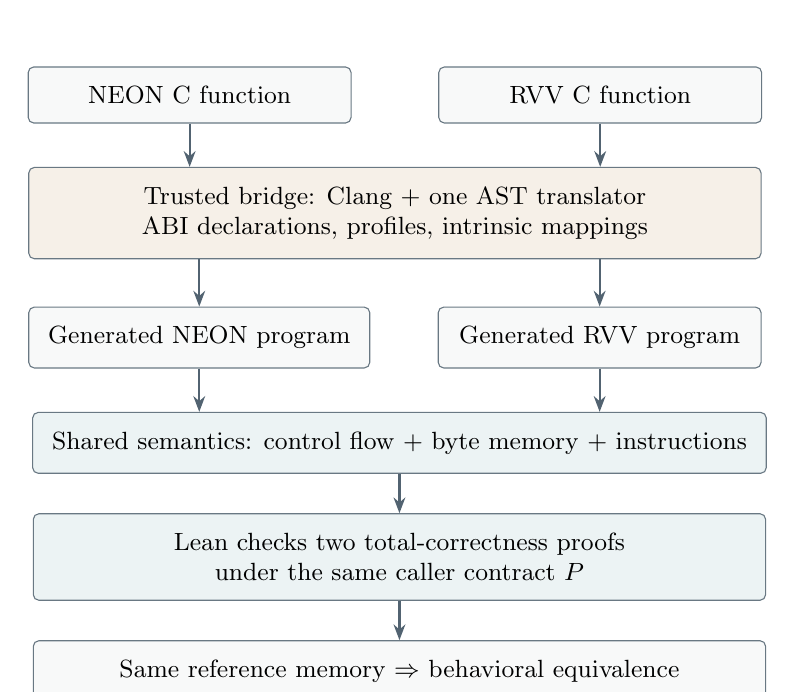
\begin{tikzpicture}[node distance=0.5cm and 1.1cm]
\node[box,minimum width=4.1cm] (nc) {NEON C function};
\node[box,minimum width=4.1cm,right=of nc] (rc) {RVV C function};
\node[box,fill=amber!10,minimum width=9.3cm,below=0.55cm of $(nc.south)!0.5!(rc.south)$] (ext) {Trusted bridge: Clang + one AST translator\\ABI declarations, profiles, intrinsic mappings};
\draw[arr] (nc)--(nc|-ext.north);\draw[arr] (rc)--(rc|-ext.north);
\node[box,minimum width=4.1cm,below=0.6cm of ext.south west,anchor=north west] (np) {Generated NEON program};
\node[box,minimum width=4.1cm,below=0.6cm of ext.south east,anchor=north east] (rp) {Generated RVV program};
\draw[arr] (ext.south-|np.north)--(np);\draw[arr] (ext.south-|rp.north)--(rp);
\node[box,fill=teal!8,minimum width=9.3cm,below=0.55cm of $(np.south)!0.5!(rp.south)$] (model) {Shared semantics: control flow + byte memory + instructions};
\draw[arr] (np)--(np|-model.north);\draw[arr] (rp)--(rp|-model.north);
\node[box,fill=teal!8,minimum width=9.3cm,below=of model] (proof) {Lean checks two total-correctness proofs\\under the same caller contract $P$};
\draw[arr] (model)--(proof);
\node[box,minimum width=9.3cm,below=of proof] (result) {Same reference memory $\Rightarrow$ behavioral equivalence};
\draw[arr] (proof)--(result);
\end{tikzpicture}
\caption{The source-to-proof boundary. One frontend produces two distinct programs. Lean checks their proofs relative to the shared definitions; it does not prove that Clang, the extractor, or the chosen definitions faithfully represent C and the architectures. The reference result and caller contract are also definitions that require review.}
\label{fig:architecture}
\end{figure}

The extractor accepts a restricted language and rejects syntax outside it. Its checks cover function shape, scalar and vector types, intrinsic declarations and signatures, initialization, and the permitted preprocessor directives. For example, a variable initialized on just one branch is not treated as definitely initialized after that branch. Selected patterns such as packing post-increments and reduction mask tables have narrow, explicit lowering rules. This is a deliberately incomplete frontend, not a general C compiler.

Per-family profiles remain necessary, but they are data: entry names, argument signatures, enabled features, directive policies, and output names. Intrinsic mappings and ABI layout information are shared tables. The old per-family scripts are compatibility entry points that delegate to the same driver; they no longer implement separate lowering algorithms. Profiles and declaration headers still affect the trusted bridge and must be audited along with its code.

Generated artifacts record hashes of their source and shared extraction inputs, the Clang version and flags, and the transitive real-header dependencies. This makes stale or mismatched artifacts detectable. A hash is provenance evidence, not a proof that the translation is semantically correct.

\subsection{What is shared, and what stays specific}
The executable machine represents local variables, memory, and pending statements. Statements perform assignments, control flow, loads, stores, assertions, and intrinsic operations. Loops unfold by ordinary steps. A failed modeled operation produces an explicit fault rather than an arbitrary successful value.

The memory layer composes little-endian words from bytes and checks read and write permissions. Addresses are 64-bit words; caller predicates establish the nonwrapping spans needed by the proofs. Shared instruction definitions provide fixed-width arithmetic, signed and unsigned interpretation, saturation, shifts, widening, narrowing, selection, and reductions. \emph{Wrapping} keeps the low bits; \emph{saturation} clips to the destination type's range. A \emph{widening} operation computes in a larger element type before a later narrowing step. The model includes the rounding modes needed by the extracted programs, rather than claiming complete coverage of every instruction mode.

A quantized activation's scale, zero point, and sequence of operations are not ISA definitions. They belong in its reference specification, built from the shared instruction primitives. Likewise, the meaning of a packed weight layout belongs in a packing specification, while the meaning of a 32-bit store belongs in the memory model. This division keeps the trusted semantic core reusable without pretending that all kernels compute the same function.

The repository enforces this separation. The \code{Model} modules contain shared definitions; \code{Spec} contains caller contracts and reference calculations; \code{Generated} contains extracted programs. Proof support lives in \code{Proofs}, and \code{Results} exposes the final claims. Model and specification modules cannot import proofs or generated programs. During the unification, the 22 extracted program bodies and the public result declarations were preserved, and nine universal specialization lemmas checked that the refactored SIMD adapters reduce to the previous arithmetic formulas.

This is an intrinsic-C semantic model. A separate assembly-like prototype exists, but the suite's established results do not use it. The trusted connection includes C object validity, ABI layouts, and intrinsic interpretation; the actual compiler and executable binaries lie beyond the current proof boundary.

\section{How a finite proof covers unbounded loops}
\subsection{Proving each program against one reference}
The main proof rule is simple: if both programs always terminate with the same reference result on the admitted inputs, they are behaviorally equivalent. The two termination proofs are independent. They need not align instructions or execute the same number of loop iterations.

For a pointwise kernel, a typical invariant says that a prefix of the output already equals the reference, the unprocessed input is still available, pointers and remaining counts describe the same suffix, and memory outside the completed stores is preserved. Figure~\ref{fig:induction} illustrates one target iteration. If $r$ elements remain, its active length $k$ satisfies $0<k\le r$ and the configured capacity bound. The instruction lemmas establish the next $k$ answers; memory lemmas combine the stores with the existing prefix. Since the new remainder is $r-k<r$, induction proves termination for every admitted initial count.

\begin{figure}[htbp]
\centering
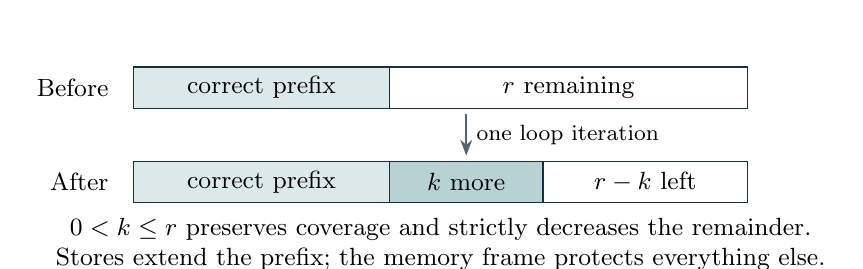
\begin{tikzpicture}[x=0.65cm,y=0.75cm,font=\small]
\node[anchor=east] at (-0.3,1.3) {Before};
\filldraw[fill=teal!15,draw=ink] (0,0.95) rectangle (5,1.65);
\filldraw[fill=white,draw=ink] (5,0.95) rectangle (12,1.65);
\node at (2.5,1.3) {correct prefix};\node at (8.5,1.3) {$r$ remaining};
\node[anchor=east] at (-0.3,-0.3) {After};
\filldraw[fill=teal!15,draw=ink] (0,-0.65) rectangle (5,0.05);
\filldraw[fill=teal!30,draw=ink] (5,-0.65) rectangle (8,0.05);
\draw[ink] (8,-0.65) rectangle (12,0.05);
\node at (2.5,-0.3) {correct prefix};\node at (6.5,-0.3) {$k$ more};
\node at (10,-0.3) {$r-k$ left};
\draw[arr] (6.5,0.85)--node[right,font=\footnotesize] {one loop iteration} (6.5,0.15);
\node[align=center] at (6,-1.35) {$0<k\le r$ preserves coverage and strictly decreases the remainder.\\Stores extend the prefix; the memory frame protects everything else.};
\end{tikzpicture}
\caption{The induction argument, shown schematically rather than as a hardware lane allocation. A proof quantifies over every progressing vector-length choice allowed by its contract; it does not enumerate a finite set of loop counts.}
\label{fig:induction}
\end{figure}

The source proof handles its fixed blocks and tail branches with its own invariant. Finite instruction blocks can be evaluated with a concrete fuel amount inside the proof. That local calculation is not a global bound on the function: induction composes arbitrarily many such blocks, up to the count and address limits stated in the contract. Here ``unbounded'' means no fixed verification unrolling bound, not that a 64-bit machine admits infinitely large arrays.

RVV tails need particular care. An inactive lane is outside the current active length, but it is not always irrelevant to later instructions. Some reductions preserve inactive accumulator lanes and eventually reduce the full accumulator. Their proofs must retain those values, not replace every inactive lane by zero. Capacity lower bounds are stated where an algorithm requires them; arbitrary positive progress alone is not sufficient for every family.

\subsection{Supporting proof infrastructure}
The generic behavior layer proves uniqueness of terminal results and stability under extra fuel. It also supports a second route: finite-path simulations. A source step may correspond to several target steps; matching terminal outcomes then gives one direction of outcome preservation. Simulations in both directions imply equivalence, including divergence agreement. This rule is available for future proofs, but the established suite primarily uses the shared total-reference rule described above.

The proof kernel checks the resulting Lean terms. The audit reports only Lean's standard principles \code{propext}, \code{Quot.sound}, and \code{Classical.choice}; it does not rely on an unchecked native execution oracle to establish the pair theorems. Executable regressions provide a separate check on definitions and generated programs. They are useful evidence, but do not replace induction or enlarge a theorem's domain.

\section{Case study: quantized arithmetic}
Quantized kernels encode values with integer zero points and multipliers. Their intended real-number operation is not precise enough to specify their bit-level behavior: wrapping, rounding, and saturation occur at specific intermediate widths. The specifications therefore describe these steps explicitly.

For signed-byte conversion, let $z_i$ and $z_o$ be the input and output zero points narrowed to 16 bits, and let $m$ be the effective 16-bit multiplier. The lane calculation has the form
\[
 d=\operatorname{wrap}_{16}(z_i-x),\qquad
 t=\operatorname{wrap}_{16}(128d),\qquad
 y=\operatorname{sat}_{8}\!\left(
    \operatorname{sat}_{16}(\operatorname{SQRDMULH}_{16}(t,m)+z_o)\right).
\]
Here SQRDMULH is signed saturating rounding doubling multiply-high: it forms the scaled high part of a product with rounding and saturation. The effective multiplier is obtained through the source's scalar negation and narrowing, so the caller contract must also make that negation defined.

A discovered translation bug doubled a product in 32 bits before narrowing. At $t=m=-32768$, the mathematical doubled product is $2^{31}$ and overflows that intermediate signed width. In a concrete conversion witness, the old target produced $-128$ where the source produced $127$. The repaired target keeps the undoubled widening product and uses a rounded narrowing shift by 15 with round-to-nearest, ties-up (RNU). The lane proof connects this sequence to the source operation; the complete conversion theorem then handles parameters, loops, tails, and memory.

Leaky ReLU adds a sign-dependent multiplier. The choice must be made from the correct intermediate value, before the subsequent shift; a branch or bit-mask identity alone is insufficient if it tests a different value. Its contract also accounts for both eagerly computed scalar multiplier negations, even when a particular lane selects only one of them.

Signed and unsigned addition expose a different mismatch. The source interprets the low byte of a negated scalar shift as a signed count $s$. Counts with $|s|\ge32$ produce zero; negative counts select a rounded right shift; nonnegative smaller counts select a wrapping left shift. Applying an RVV shift directly would instead mask the count to the element width and could turn a large shift into a small one. The repair explicitly decodes the source count and selects the appropriate target path. In the unsigned case, subtracting zero points must still preserve negative differences by widening into a signed intermediate type.

These examples explain why the unified model contains reusable width and rounding operations while the specifications retain family-specific compositions. The signed and unsigned addition proofs cover all admitted parameter values, not just the counterexamples that motivated the repairs. The raw scalar negation must remain defined; vector wrapping does not justify accepting \code{INT32\_MIN} for that negated parameter.

\section{Case study: row sums across two dimensions}
The row-sum family is a useful stress test because both the row count and channel count drive loops. For $R$ rows, $C$ channels, input base $I$, row stride $S$, and output base $O$, the reference updates output word $j$ to
\[
 \mathit{out}'_j=\mathit{out}_j+
 \sum_{i=0}^{R-1}\operatorname{interpret}(M[I+iS+j])\pmod{2^{32}},
 \qquad 0\le j<C.
\]
The signed version interprets each input byte in $[-128,127]$; the unsigned version uses $[0,255]$. All inputs and old output values come from the initial memory $M$. Other bytes and permissions remain unchanged.

Both implementations organize work using groups of seven rows, substituting a zero buffer for absent rows in a final group. The source also bounds each accumulation batch to at most 252 rows before resetting its halfword accumulators, preventing overflow at that intermediate width. It processes channel blocks and then smaller tails. The target uses its own row setup and variable-length channel strips, widening the accumulated values to 32-bit output words. A proof must connect both loop nests to the same rectangular sum; proving only a seven-row body leaves the outer loops unjustified.

\begin{figure}[htbp]
\centering
\begin{minipage}[t]{0.48\linewidth}
\centering
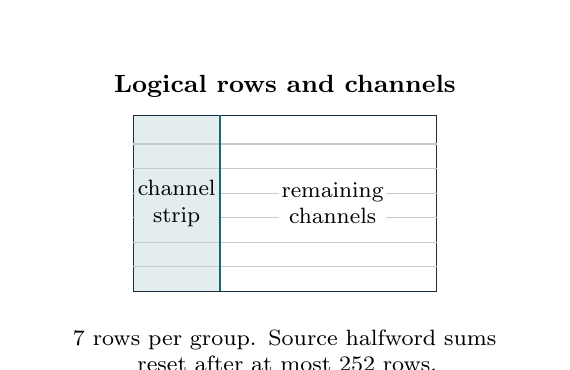
\begin{tikzpicture}[font=\small,x=0.11cm,y=0.52cm]
\node[align=center,text width=6.3cm,font=\bfseries\small] at (17.5,5.5) {Logical rows and channels};
\fill[teal!12] (0,0.5) rectangle (10,4.8);
\draw[ink] (0,0.5) rectangle (35,4.8);
\foreach \y in {1.1,1.7,2.3,2.9,3.5,4.1} {\draw[ink!25] (0,\y)--(35,\y);}
\draw[teal,thick] (10,0.5)--(10,4.8);
\node[align=center,font=\footnotesize,fill=teal!12,inner sep=1pt] at (5,2.65) {channel\\strip};
\node[align=center,font=\footnotesize,fill=white,inner sep=1pt] at (23,2.65) {remaining\\channels};
\node[anchor=north,align=center,text width=6.3cm,font=\footnotesize] at (17.5,-0.2) {7 rows per group. Source halfword sums\\reset after at most 252 rows.};
\end{tikzpicture}
\end{minipage}\hfill
\begin{minipage}[t]{0.48\linewidth}
\centering
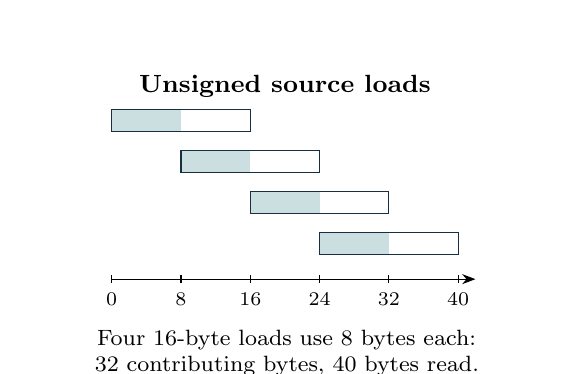
\begin{tikzpicture}[font=\small,x=0.11cm,y=0.52cm]
\node[align=center,text width=6.3cm,font=\bfseries\small] at (20,5.5) {Unsigned source loads};
\foreach \offset/\y in {0/4.4,8/3.4,16/2.4,24/1.4} {
 \fill[teal!22] (\offset,\y) rectangle +(8,0.55);
 \draw[ink] (\offset,\y) rectangle +(16,0.55);
}
\draw[-{Stealth}] (0,0.8)--(42,0.8);
\foreach \x in {0,8,16,24,32,40} {\draw (\x,0.7)--(\x,0.9);\node[below,font=\scriptsize] at (\x,0.7) {\x};}
\node[anchor=north,align=center,text width=6.3cm,font=\footnotesize] at (20,-0.2) {Four 16-byte loads use 8 bytes each:\\32 contributing bytes, 40 bytes read.};
\end{tikzpicture}
\end{minipage}
\caption{Two distinct obligations in row reduction. Left: row grouping and channel strip processing must cover the whole logical matrix. Right: bytes that do not contribute to the sum can still be loaded. The shaded halves contribute; every outlined byte must be readable, including when the pointer is replaced by the zero buffer.}
\label{fig:rows}
\end{figure}

The caller contract makes these obligations explicit. It admits $0<R<2^{31}$ and $0<C<2^{64}$, with nonwrapping address calculations, including $7S<2^{64}$. Each row has $C+15$ readable bytes. The zero buffer contains at least $\max(C,40)$ readable zero bytes. Output words are aligned, readable, writable, and separated from the padded row regions and the zero buffer. Rows may overlap one another because they are read-only.

The 40-byte zero-buffer requirement is easy to miss. In an unsigned source block, four 16-byte loads begin at offsets 0, 8, 16, and 24, although only the low eight bytes from each load contribute. Figure~\ref{fig:rows} separates the mathematical contribution from the actual footprint. A specification based only on the former would silently admit invalid executions.

The signed source has another asymmetry: its final odd channel uses scalar signed addition. The sum of the old output word and the signed interpretation of the modular column sum must fit in 32 bits on that path. Vector additions elsewhere retain their wrapping semantics; the unsigned scalar path wraps as well. A guarded scalar conversion through double and floor also remains part of the trusted frontend interpretation, with exactness justified only over this contract's domain, not for arbitrary floating-point inputs.

The proofs induct over both row batches and channel strips, maintain intermediate range bounds, and compose the resulting stores with the memory frame. Compiled Lean regressions exercise rows 251, 252, 253, 504, and 505, selected channel counts through 65, and multiple vector capacities. These tests probe reset and tail boundaries; the universal claims come from the proofs. Neither row-sum target needed repair, and these regressions are executions of the Lean model, not a native C row-sum experiment.

\section{Established results and their boundaries}
Table~\ref{tab:coverage} summarizes the 11 complete pair proofs. Each has a common behavioral-equivalence theorem, separate source and target return theorems, and a witness that its caller predicate is inhabited. The witness rules out a trivially empty contract; it does not establish that every application caller satisfies that contract.

\begin{table}[htbp]
\centering\small
\begin{tabular}{@{}p{0.26\linewidth}p{0.34\linewidth}p{0.34\linewidth}@{}}
\toprule
Family and pair count & Exact reference behavior & Material contract conditions \\
\midrule
Signed clamp (1) & Signed-byte pointwise clamp & Ordered narrowed bounds; padded input; separate output \\[5pt]
Signed conversion and leaky ReLU (2) & Width-specific rounded, saturating lane calculations & Readable parameters; defined eager scalar negations \\[5pt]
Signed / unsigned addition (2) & Products, decoded shift, saturation, output clamp & Inputs may alias each other; output separate; defined shift negation \\[5pt]
Word transpose (1) & Original word $(r,c)$ copied to $(c,r)$, including zero-dimension cases & Aligned, nonwrapping layouts; input padding and output separation \\[5pt]
Grouped weight packing (1) & Two-channel tiles, optional bias, preserved holes and gaps & Positive dimensions; aligned separated output; capacity at least eight \\[5pt]
Signed / unsigned scalar byte sums (2) & Original byte sum added to old output word & Input/output overlap allowed; signed scalar addition defined; capacity at least eight \\[5pt]
Signed / unsigned row sums (2) & Original column sums added to old output words & Padded rows and zero storage; separate output; signed odd-tail condition \\
\bottomrule
\end{tabular}
\caption{Whole-function proof coverage: 11 of 36 implemented pairs. These are summaries of the caller domains, not substitutes for the full formal predicates. All results specify the complete final memory.}
\label{tab:coverage}
\end{table}

Several less obvious behaviors are preserved intentionally. In transpose, zero height skips the work, but zero width with positive height still copies the first column in the source. The repaired target follows that behavior. In weight packing, a null bias pointer writes zero headers; an odd final channel with a present bias leaves the absent channel's header unwritten. Odd-channel weight holes and extra-byte gaps between tiles also remain unchanged. An output-array-only comparison could overlook these distinctions.

Scalar byte sums require a different invariant from row sums. The source accumulates blocks of up to 2048 bytes into halfwords, using bounds such as $[-32768,32512]$ for signed partial sums and $[0,65280]$ for unsigned ones. Its tail uses a mask table and up to 15 readable padding bytes. The target preserves inactive accumulator lanes and reduces the full accumulator at the end. All reads precede the single final store, which is why overlapping input and output can be admitted for this family.

The manifest contains 40 source entries. Three targets are absent: \code{qd8-f32-qc8w-gemm-minmax}, \code{qd8-f32-qc8w-igemm-minmax}, and \code{qs8-qc8w-gemm-minmax-fp32}. The \code{u8-vclamp} target is empty. These four are excluded under the clarified scope. Of the 36 implemented pairs, 25 still lack whole-function proofs. In particular, the development does not claim full floating-point kernel equivalence. This report preserves that distinction rather than extrapolating from the proved integer families.

\section{Translation repairs and the strength of their evidence}
The audit repaired 17 existing targets. Four repaired targets also have complete pair proofs: signed conversion, word transpose, and signed and unsigned addition. For the other repairs, evidence consists of targeted regressions and, where available, isolated operation lemmas. Table~\ref{tab:repairs} records the failure mechanisms and changes; full counterexamples and code details are retained in the repository's repair log.

\begin{table}[htbp]
\centering\small
\begin{tabular}{@{}p{0.25\linewidth}p{0.69\linewidth}@{}}
\toprule
Targets (count) & Observed mismatch and repair \\
\midrule
Signed conversion (1) & Doubling overflowed before narrowing. Keep the widening product undoubled and apply an RNU narrowing shift by 15. \\[5pt]
Word transpose (1) & The target skipped a zero-width, positive-height case that the source executes. Match the source's dimension guards. \\[5pt]
Signed / unsigned add (2) & Masked RVV shift counts differed from the source's signed low-byte counts. Decode direction and out-of-range cases explicitly. \\[5pt]
Floating depthwise convolution (1) & Packed weights use stride four even in a tail. Preserve that stride and cap each tile at four. \\[5pt]
Floating sparse matrix multiply (1) & Fused arithmetic and pointer progression differed. Match the source FMA, its 4/2/1 strips, and carried offsets. \\[5pt]
Floating exponential-sum reduction (1) & Reassociation changed the result. Preserve four accumulator chains, pairwise grouping, and 2/1 tail order. \\[5pt]
Seven binary floating kernels and square root (8) & Default NaN results lost source priority or payload. Restore the source's signaling/quiet selection and quieting behavior. \\[5pt]
Quantized multiply via float (1) & A shortcut missed magic-bias rounding and NaN behavior. Restore float addition, bit reinterpretation, saturating subtraction, and scale propagation. \\[5pt]
Floating HWC-to-CHW convolution (1) & Loading before merging still touched inactive addresses. Use genuinely masked strided loads. \\
\bottomrule
\end{tabular}
\caption{Seventeen repaired targets. The seven binary floating kernels are add, subtract, multiply, divide, minimum, maximum, and multiply-by-constant. Repair count and proof coverage measure different things.}
\label{tab:repairs}
\end{table}

Small examples make two floating-point issues concrete. Consider
\[ a=\texttt{0x1.000002p0},\qquad w=\texttt{0x1.fffffcp-1},\qquad b=-1. \]
A fused multiply-add $aw+b$ gives $-2^{-46}$ while separate rounded multiply and add give zero. Similarly, one exponential-reduction witness with inputs $[0,-17,\ldots,-17]$ and maximum zero gives \texttt{0x1.000004p+0} under the source's grouping and \texttt{0x1p+0} under sequential accumulation. Neither difference can be repaired by proving equality over real arithmetic.

NaNs require a separate account. In the modeled ARM behavior, the first signaling NaN takes priority; otherwise the first quiet NaN does. The selected payload is quieted and preserved. A lemma proves that the repair's sequence of merges implements this selection rule. That lemma concerns the NaN subexpression, not all arithmetic, loops, and memory behavior of the surrounding floating-point kernels.

Five C regression programs compare actual repository NEON kernels executed natively on AArch64 with RVV targets executed through an intrinsic interpreter. The floating-point environment uses round-to-nearest, ties-to-even, gradual underflow, and payload propagation (FPCR zero), with compiler contraction disabled except where an explicit intrinsic requires fused behavior. Tests use VLEN 128, 256, and 512 and exercise boundary lengths, special floating-point words, all 256 effective shift counts, and allocation-edge masked loads. AddressSanitizer and UndefinedBehaviorSanitizer check the tested executions. Real-header code-generation checks also compile all 17 repaired targets for RVV. These checks detect concrete discrepancies and signature errors; they do not prove correctness of the interpreter, compiler, or generated binaries.

A separate cvc5-backed adapter regression checks that inactive masked-load addresses are not read and that preserved lanes retain their values. The older Bitwuzla adapter was not changed. This targeted adapter check should not be read as a new whole-pipeline symbolic-verification guarantee.

\section{Trust, reproducibility, and remaining work}\label{sec:reproduce}
The trusted computing base has two different roles. Lean's kernel and standard logical principles validate proof terms. Separately, the source-to-model bridge and the human interpretation of the definitions determine what those terms say about the repository's C programs. Clang, the shared extractor, its profiles and declaration headers, ABI tables, and intrinsic mappings are in that second category. Unifying the frontend reduces duplicated logic; it does not remove this trust obligation.

The semantic definitions and caller predicates also require scrutiny. A perfectly checked proof of a weak output specification or an unnecessarily restrictive caller predicate would still be a weak result. Full-memory observations, explicit permission preservation, nonempty caller witnesses, and audits of exact theorem types help expose these issues, but no automated check replaces reviewing the intended meaning. Floating-point operation order, NaN behavior, architectural flags, object lifetime, and compiler behavior are especially important boundaries for future work.

The reproducible check suite regenerates the extracted programs, runs 66 frontend tests and six layout tests, builds Lean, executes model regressions, audits theorem types and dependencies, checks target compilation, and runs the repair experiments. The recorded checks passed after the frontend/model refactor. The dependency audit reported only the standard Lean principles listed in Section 4. The strict completeness option intentionally fails because 25 implemented pairs remain unproved; the coverage report does not hide those entries.

For a reader continuing the work, the following entry points connect the paper to the artifacts:
\begin{center}\small
\begin{tabular}{@{}p{0.43\linewidth}p{0.51\linewidth}@{}}
\toprule
Artifact & Purpose \\
\midrule
\code{verification/README.md} & Setup, architecture, and check commands \\
\code{verification/extraction/README.md} & Supported frontend and trust boundary \\
\code{Salty/Specifications.lean} & Definition-only entry to the formal specifications \\
\code{Salty/Results/} & Final pair claims and caller-domain witnesses \\
\code{verification/coverage.json} & Source provenance and proof coverage \\
\code{verification/REPAIRS.md} & Counterexamples, edits, and repair evidence \\
\bottomrule
\end{tabular}
\end{center}
The \code{Salty} paths are relative to \code{verification/lean}. The development pins Lean 4.21.0-rc3 and uses Std without Mathlib. From the repository root, the full check command is
\begin{quote}\small\ttfamily
RISCV\_CLANG=/path/to/riscv-capable/clang \textbackslash{}\\
CVC5\_PREFIX=/path/to/cvc5-sdk \textbackslash{}\\
python3 verification/run\_checks.py
\end{quote}
The native regression portion requires the documented AArch64 environment and SDKs. The report itself is built with \code{python3 verification/report/build.py}. No Lean agent was added to the translation pipeline; this development is a reusable verification foundation and a checked suite of existing cases.

The next substantial proof work is in the 25 remaining implemented pairs, especially floating-point arithmetic and larger loop nests. An assembly-level connection would further reduce the gap between the verified model and execution, but requires a new correspondence argument rather than a change of terminology. Performance effects of the repairs have not been measured; preserving source grouping can constrain vector utilization.

\section{Conclusion}
Whole-function SIMD equivalence requires arithmetic, control flow, memory safety, and caller assumptions to fit together. The shared model makes those obligations explicit, while independent proofs against one reference let NEON and RVV retain different execution schedules. Eleven pairs now have termination and exact-memory guarantees for all admitted calls without a fixed unrolling bound. The remaining coverage and trust boundaries are explicit, and the repair evidence is kept separate from universal proof claims. This separation makes the framework useful both for extending verification and for understanding exactly what has already been established.

\label{body-end}
\clearpage
\section*{References}
\small
The architectural documents below provide context for the chosen semantics. They are not imported as machine-checked proofs of the source-to-model correspondence.
\begin{enumerate}
\item Leonardo de Moura et al. \emph{Theorem Proving in Lean 4}. Lean documentation. \url{https://lean-lang.org/theorem_proving_in_lean4/}
\item Arm. \emph{Arm NEON Intrinsics Reference}. Advanced SIMD intrinsic definitions. \url{https://arm-software.github.io/acle/neon_intrinsics/advsimd.html}
\item RISC-V International. \emph{The RISC-V Instruction Set Manual, Volume I: Vector Extension, Version 1.0}. \url{https://docs.riscv.org/reference/isa/unpriv/v-st-ext}
\item RISC-V International. \emph{Single-Precision Floating-Point Extension, Version 2.2}. \url{https://docs.riscv.org/reference/isa/unpriv/f-st-ext.html}
\item RISC-V International. \emph{RISC-V Vector C Intrinsics, Version 1.0}. Includes fixed-point rounding controls. \url{https://docs.riscv.org/reference/vector-c-intrinsics/v1.0/rvv-intrinsic-spec.html}
\item Arm. \emph{Arm Architecture Reference Manual Supplement: Morello for A-profile Architecture}, DDI 0606 A.j, sections 5.539--5.540, \code{FPProcessNaN}/\code{FPProcessNaNs}. Arm-authored document, mirrored at \url{https://kib.kiev.ua/x86docs/ARM/Morello/DDI0606_A.j_morello_architecture_external.pdf}.
\item Arm. \emph{Procedure Call Standard for the Arm 64-bit Architecture}, Section 6.1.2. \url{https://github.com/ARM-software/abi-aa/blob/main/aapcs64/aapcs64.rst}
\item SALTy-rn repository artifacts, 14 October 2026: the coverage manifest, repair log, extracted programs, and Lean specifications and results listed in Section~\ref{sec:reproduce}. The manifest records the exact source hashes associated with the established coverage.
\end{enumerate}
\end{document}
